\section{Application to Bosonic Encodings}
\label{sec4}
\begin{figure*}[t]
    \centering
    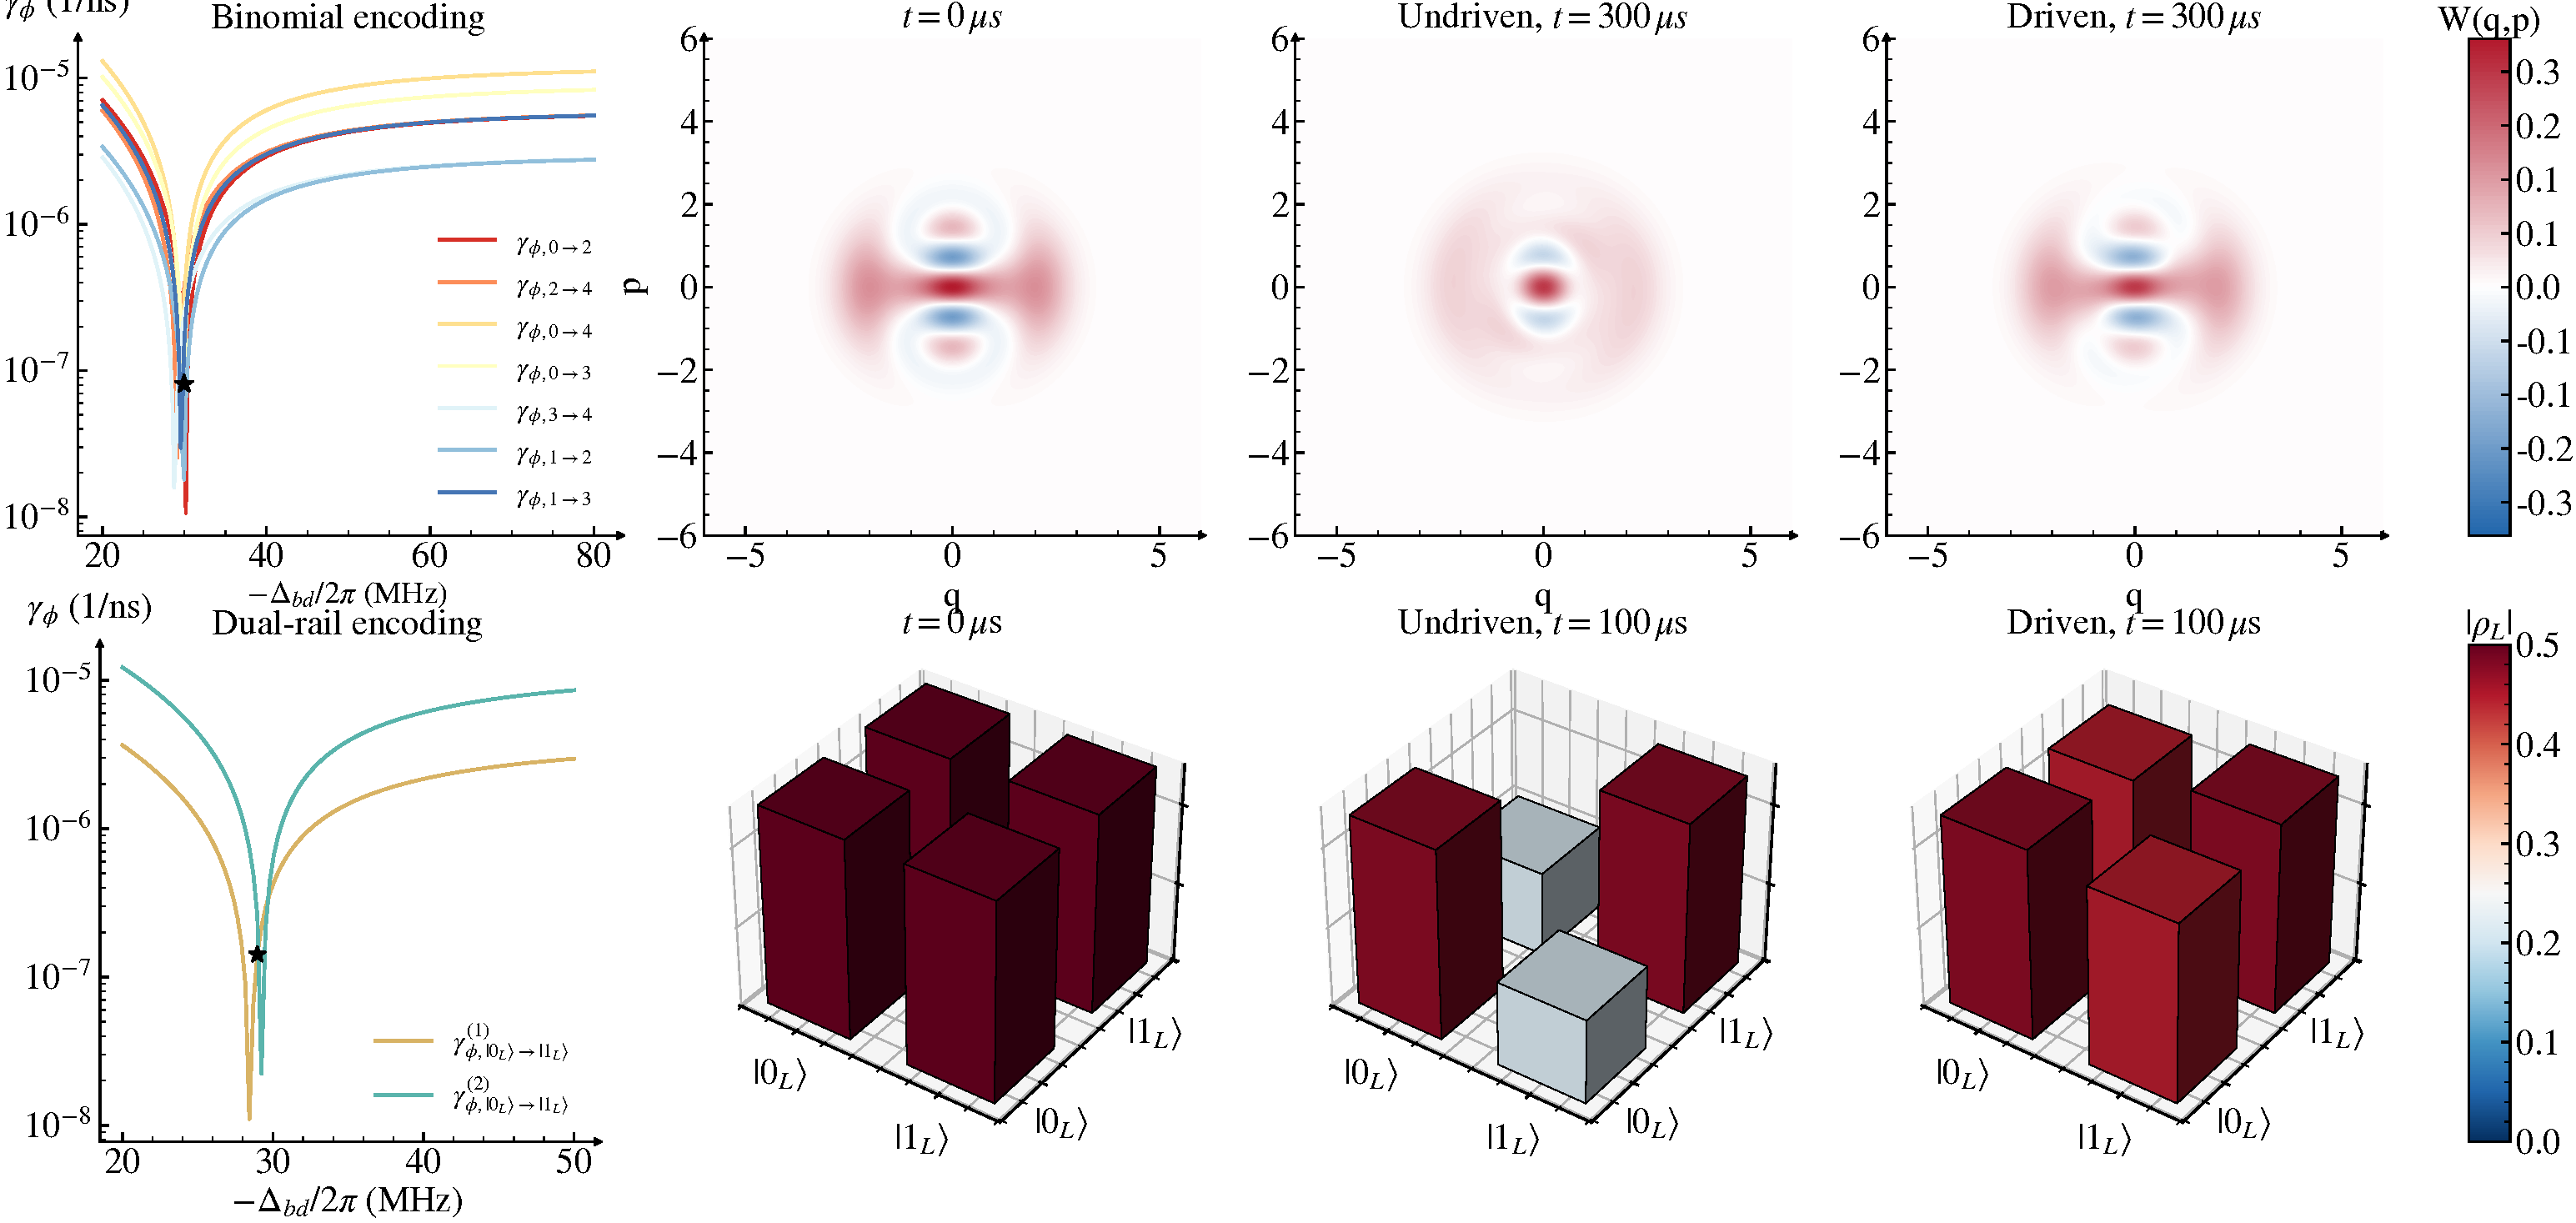
\includegraphics[width=\textwidth]{Sec4/qec_plot.pdf}
    \caption{\textbf{Driven sweet-spot protection for bosonic encodings} (\(\Omega_0/2\pi=10\,\mathrm{MHz}\) throughout).
    \emph{Binomial code}---\textbf{(a)}~Dephasing rate \(\gamma_{\phi,n\rightarrow m}\) of cavity transitions due to FTT-frequency fluctuations as a function of \(\Delta_{bd}\); the star marks \(\Delta_{bd}/2\pi=-30\,\mathrm{MHz}\), where all relevant \(\gamma_{\phi,n\rightarrow m}\) are suppressed by at least \(\sim\!13\times\).
    \textbf{(b)}~Wigner function of \(|+_L\rangle\) at \(t=300\,\mu\mathrm{s}\): the driven case retains the interference fringes that are lost without the drive.
    \emph{Dual-rail encoding}---\textbf{(c)}~Dephasing rate \(\gamma_{\phi,0\rightarrow 1}^{(i)}\) for each cavity as a function of \(\Delta_{bd}\); both cavities exhibit \(\sim 10\times\) lower dephasing near \(-\Delta_{bd}/2\pi\sim 29\,\mathrm{MHz}\).
    \textbf{(d)}~Logical-subspace tomography for one dual-rail qubit: the drive suppresses dephasing, while leakage from single-photon loss remains unchanged.}
\label{fig:qec_plot}
\end{figure*}

In the previous sections, we showed that operating at a driven sweet spot can extend the cavity dephasing time by more than an order of magnitude. Here we apply the same strategy to bosonic quantum error correction (QEC). The central observation is that, in the unselective regime, the drive does not resolve individual photon-number states, so a single choice of drive parameters simultaneously suppresses the dephasing rates of all relevant cavity transitions induced by FTT-frequency fluctuations. This property is precisely what is needed for bosonic encodings, which store quantum information in superpositions of multiple Fock states.

Throughout this section, we fix the drive amplitude at $\Omega_0/2\pi=10~\mathrm{MHz}$ and sweep the detuning $\Delta_{bd}$ to identify the operating point that simultaneously minimizes the relevant dephasing rates. The metrics below---transition dephasing rates and logical-subspace coherence proxies---quantify the suppression of inherited dephasing rather than a full logical error rate, which would additionally require modeling the complete QEC cycle.

\subsection{Binomial encoding}
As a concrete example, consider the minimal binomial code \cite{Michael2016}
\begin{equation}
|0_L\rangle=\frac{|0\rangle+|4\rangle}{\sqrt{2}},\qquad |1_L\rangle=|2\rangle,
\end{equation}
the simplest binomial encoding that corrects a single photon-loss event. The drive is not intended to eliminate all dephasing; rather, it suppresses the specific transition-frequency fluctuations that dominate the logical-phase diffusion and recovery-sensitive coherences for this encoding. We now identify these transitions explicitly.

For the logical basis state \( |0_L\rangle \propto |0\rangle + |4\rangle \), fluctuations of the \(0\!\rightarrow\!4\) splitting, \( \delta\widetilde{\omega}_{c,0\rightarrow 4}(t) \), induce phase diffusion between \( |0\rangle \) and \( |4\rangle \) and therefore deform \( |0_L\rangle \).
Because this code does not protect against pure dephasing, the coherence of an arbitrary superposition \( \alpha|0_L\rangle + \beta|1_L\rangle \) is carried by the bare-state coherences \( |0\rangle\!\leftrightarrow\!|2\rangle \) and \( |2\rangle\!\leftrightarrow\!|4\rangle \). Suppressing the corresponding dephasing rates \(\gamma_{\phi,0\rightarrow 2}\) and \(\gamma_{\phi,2\rightarrow 4}\) therefore directly improves logical coherence.

After a single photon loss, the code space maps as \( |0_L\rangle \rightarrow |3\rangle \) and \( |1_L\rangle \rightarrow |1\rangle \), so the logical information temporarily resides in the \( |1\rangle\!\leftrightarrow\!|3\rangle \) coherence prior to correction. Suppressing \(\gamma_{\phi,1\rightarrow 3}\) is thus essential for high-fidelity recovery. During the recovery itself, intermediate superpositions populate the \(\{|0\rangle,|3\rangle,|4\rangle\}\) manifold and the \(\{|1\rangle,|2\rangle\}\) manifold, making the corresponding transition dephasing rates---e.g., \(\gamma_{\phi,0\rightarrow 3}\), \(\gamma_{\phi,3\rightarrow 4}\), and \(\gamma_{\phi,1\rightarrow 2}\)---additional targets for suppression.

To quantify the improvement, we sweep the detuning \(\Delta_{bd}\) at fixed \(\Omega_0/2\pi = 10\,\mathrm{MHz}\) and evaluate the dephasing rate due to flux noise,
\begin{equation}
\gamma_{\phi,{n\rightarrow m}}= S_0\bigg|\frac{\partial \widetilde{\omega}_{c,n\rightarrow m}}{\partial \Phi}\bigg|\sqrt{2\ln(|\omega_\text{ir}t|)}.
\end{equation}
Here, \(\omega_\text{ir}\) is the infrared cutoff of the \(1/f\) noise spectrum (set by the inverse of the total measurement time) and \(t\) is the experimental timescale. An earlier experiment reported \(\ln(|\omega_\text{ir} t|)\approx 4\) \cite{PhysRevX.7.031037factor4}, and we use this value in the following numerics. The results are shown in Fig.~\ref{fig:qec_plot}(a). The minima of several dephasing rates overlap near \(-\Delta_{bd}/2\pi \simeq 30\,\mathrm{MHz}\), consistent with the unselective regime \(\Delta_{bd}\gg |\chi|\) (here \(|\chi|/2\pi \sim 0.5\,\mathrm{MHz}\)).

Choosing \(\Delta_{bd}/2\pi = -30\,\mathrm{MHz}\) yields a worst-case reduction of the dephasing rate by a factor of \(\sim 13\) across the relevant transitions. This improvement is confirmed by Wigner tomography [Fig.~\ref{fig:qec_plot}(b)], which serves as a direct proxy for the preservation of coherence within the logical subspace. For the initial state \(|+_L\rangle = (|0_L\rangle + |1_L\rangle)/\sqrt{2}\), the undriven Wigner function reduces to a mixture of Fock states after \(300\,\mu\mathrm{s}\), indicating complete loss of logical coherence. In the driven case, the characteristic interference fringes are largely retained, confirming that the drive preserves the intra-code-word coherence required by the binomial encoding.

\subsection{Dual-rail encoding}
Dual-rail encoding is widely used because the dominant single-photon-loss error maps to a detectable erasure \cite{dualrailcavity1,teoh2023dual}. A single dual-rail qubit is encoded in two cavities with logical states \(\ket{0_L}=\ket{01}\) and \(\ket{1_L}=\ket{10}\). The fault-tolerance advantage of this encoding relies on the error hierarchy in which single-photon loss dominates over dephasing; inherited cavity dephasing from a flux-tunable coupler can degrade this bias. To implement two-qubit gates, one approach is to couple two dual-rail qubits via an FTT and exploit its three-wave-mixing interaction.

In this architecture, the FTT (mode \(b\)) couples to two cavities labeled by \(i\). Flux fluctuations \(\delta\Phi(t)\) modulate the FTT frequency, and this modulation enters the cavity spectrum through the Lamb shift, producing cavity-frequency fluctuations
\begin{equation}
\delta \widetilde{\omega}^{(i)}_{c}(t)=\biggl(\frac{g^{(i)}}{\Delta^{(i)}_{bc}}\biggr)^2\,\delta\omega_b(t),
\end{equation}
where \(g^{(i)}\) and \(\Delta^{(i)}_{bc}\) are the coupling strength and detuning between the FTT and cavity \(i\), respectively. Because each cavity forms one rail of a dual-rail qubit, these fluctuations contribute directly to logical dephasing. By appropriately driving the coupler, the dephasing rates of both cavities due to inherited FTT-frequency noise can be reduced simultaneously.

Fig.~\ref{fig:qec_plot}(c) shows the numerically computed dephasing rate \(\gamma_{\phi,0\rightarrow 1}^{(i)}\) for each cavity as \(\Delta_{bd}\) is swept. Choosing \(-\Delta_{bd}/2\pi\sim 29\,\mathrm{MHz}\) yields \(\sim 10\times\) lower dephasing rates for both cavities than in the undriven case. We then simulate the dynamics of a single dual-rail qubit and show the state tomography in the logical subspace in Fig.~\ref{fig:qec_plot}(d). The simulation confirms that the drive largely suppresses pure dephasing within the logical subspace, while single-photon-loss-induced leakage out of the logical subspace remains nearly unchanged between the driven and undriven cases. This demonstrates that the driven sweet spot acts as a bias-preserving knob: it mitigates inherited dephasing while leaving the dominant single-photon-loss channel—and hence the favorable error hierarchy of the dual-rail encoding—intact.